% Copyright 2015-2016 Dan Foreman-Mackey and the co-authors listed below.

\documentclass[manuscript, letterpaper]{aastex}

\pdfoutput=1

\include{vc}
\newcommand{\abctoytruth}{{\ensuremath{6.78}}}
\newcommand{\abctoynobs}{{\ensuremath{6}}}
\newcommand{\abctoyeps}{{\ensuremath{10^{-3}}}}
\newcommand{\abctoyS}{{\ensuremath{50}}}
\newcommand{\abctoyheuristic}{{\ensuremath{5.26^{+3.82}_{2.65}}}}
\newcommand{\abctoyabc}{{\ensuremath{5.71^{+2.71}_{2.09}}}}


\usepackage{microtype}

\usepackage{url}
\usepackage{amssymb,amsmath}
\usepackage{natbib}
\usepackage{multirow}
\bibliographystyle{aasjournal}

% ----------------------------------- %
% start of AASTeX mods by DWH and DFM %
% ----------------------------------- %

\setlength{\voffset}{0in}
\setlength{\hoffset}{0in}
\setlength{\textwidth}{6in}
\setlength{\textheight}{9in}
\setlength{\headheight}{0ex}
\setlength{\headsep}{\baselinestretch\baselineskip} % this is 2 lines in ``manuscript''
\setlength{\footnotesep}{0in}
\setlength{\topmargin}{-\headsep}
\setlength{\oddsidemargin}{0.25in}
\setlength{\evensidemargin}{0.25in}

\linespread{0.54} % close to 10/13 spacing in ``manuscript''
\setlength{\parindent}{0.54\baselineskip}
\hypersetup{colorlinks = false}
\makeatletter % you know you are living your life wrong when you need to do this
\long\def\frontmatter@title@above{
\vspace*{-\headsep}\vspace*{\headheight}
\noindent\footnotesize
{\noindent\footnotesize\textsc{\@journalinfo}}\par
{\noindent\scriptsize Preprint typeset using \LaTeX\ style AASTeX6\\
With modifications by David W. Hogg and Daniel Foreman-Mackey
}\par\vspace*{-\baselineskip}\vspace*{0.625in}
}%
\makeatother

% Section spacing:
\makeatletter
\let\origsection\section
\renewcommand\section{\@ifstar{\starsection}{\nostarsection}}
\newcommand\nostarsection[1]{\sectionprelude\origsection{#1}}
\newcommand\starsection[1]{\sectionprelude\origsection*{#1}}
\newcommand\sectionprelude{\vspace{1em}}
\let\origsubsection\subsection
\renewcommand\subsection{\@ifstar{\starsubsection}{\nostarsubsection}}
\newcommand\nostarsubsection[1]{\subsectionprelude\origsubsection{#1}}
\newcommand\starsubsection[1]{\subsectionprelude\origsubsection*{#1}}
\newcommand\subsectionprelude{\vspace{1em}}
\makeatother

\widowpenalty=10000
\clubpenalty=10000

\sloppy\sloppypar

% ------------------ %
% end of AASTeX mods %
% ------------------ %

% Projects:
\newcommand{\project}[1]{\textsl{#1}}
\newcommand{\kepler}{\project{Kepler}}
\newcommand{\ktwo}{\project{K2}}
\newcommand{\tess}{\project{TESS}}
\newcommand{\plato}{\project{PLATO}}
\newcommand{\gaia}{\project{Gaia}}

\newcommand{\accronym}[1]{\textsc{#1}}
\newcommand{\foreign}[1]{\emph{#1}}
\newcommand{\etal}{\foreign{et\,al.}}
\newcommand{\etc}{\foreign{etc.}}

\newcommand{\dfmfigref}[1]{\ref{fig:#1}}
\newcommand{\dfmFig}[1]{Figure~\dfmfigref{#1}}
\newcommand{\dfmfig}[1]{\dfmFig{#1}}
\newcommand{\dfmfiglabel}[1]{\label{fig:#1}}

% \newcommand{\Tab}[1]{Table~\ref{tab:#1}}
% \newcommand{\tab}[1]{\Tab{#1}}
\newcommand{\tablabel}[1]{\label{tab:#1}}

\renewcommand{\eqref}[1]{\ref{eq:#1}}
\newcommand{\Eq}[1]{Equation~(\eqref{#1})}
\newcommand{\eq}[1]{\Eq{#1}}
\newcommand{\eqalt}[1]{Equation~\eqref{#1}}
\newcommand{\eqlabel}[1]{\label{eq:#1}}

\newcommand{\sectionname}{Section}
\newcommand{\sectref}[1]{\ref{sect:#1}}
\newcommand{\Sect}[1]{\sectionname~\sectref{#1}}
\newcommand{\sect}[1]{\Sect{#1}}
\newcommand{\sectalt}[1]{\sectref{#1}}
\newcommand{\App}[1]{Appendix~\sectref{#1}}
\newcommand{\app}[1]{\App{#1}}
\newcommand{\sectlabel}[1]{\label{sect:#1}}

\newcommand{\T}{\ensuremath{\mathrm{T}}}
\newcommand{\dd}{\ensuremath{\,\mathrm{d}}}
\newcommand{\unit}[1]{{\ensuremath{\,\mathrm{#1}}}}
\newcommand{\bvec}[1]{{\ensuremath{\boldsymbol{#1}}}}
\newcommand{\appropto}{\mathrel{\vcenter{
  \offinterlineskip\halign{\hfil$##$\cr
    \propto\cr\noalign{\kern2pt}\sim\cr\noalign{\kern-2pt}}}}}
\newcommand{\densityunit}{{\ensuremath{\mathrm{nat}^{-2}}}}


% TO DOS
\newcommand{\todo}[3]{{\color{#2}\emph{#1}: #3}}
\newcommand{\dfmtodo}[1]{\todo{DFM}{red}{#1}}
\newcommand{\tdmtodo}[1]{\todo{TDM}{blue}{#1}}
\newcommand{\hoggtodo}[1]{\todo{HOGG}{blue}{#1}}

% Response
\newcommand{\response}[1]{{\color{blue}#1}}

% Helpers for this paper:
\newcommand{\license}{MIT License}
\newcommand{\paper}{paper}

% Notation for this paper:
\newcommand{\obs}{{\ensuremath{\mathrm{obs}}}}
\newcommand{\simu}{{\ensuremath{\mathrm{sim}}}}
\def\abc{Approximate Bayesian Computation (\accronym{abc})\def\abc{\accronym{abc}}}
\def\mcmc{Markov Chain Monte Carlo (\accronym{mcmc})\def\mcmc{\accronym{mcmc}}}

\newcommand{\datareleaseurl}{TBD}


% \shorttitle{The population of long-period transiting exoplanets}
% \shortauthors{Foreman-Mackey, Morton, Hogg, \etal}
% \submitted{Submitted to \textit{The Astrophysical Journal}}

\begin{document}

\title{%
\vspace{\baselineskip}
Approximate Bayesian Computation of the population of exoplanets
\vspace{-2\baselineskip}  % OMG AASTEX6 IS SO BROKEN
}

\newcounter{affilcounter}
\altaffiltext{1}{\textsf{danfm@uw.edu}; Sagan Fellow}

\setcounter{affilcounter}{2}
\edef \uw {\arabic{affilcounter}}\stepcounter{affilcounter}
\altaffiltext{\uw}       {Astronomy Department, University of Washington,
                          Seattle, WA, 98195, USA}

\author{%
    Daniel~Foreman-Mackey\altaffilmark{1,\uw},
    and friends
    \vspace{\baselineskip}
}


\begin{abstract}

The \kepler\ Mission was designed to statistical questions about the
population of exoplanets.
So far, all occurrence rate and distribution results have required either
strong modeling assumptions or heuristic (qualitative) inference methods.
We present a general method of occurrence rate measurement using Approximate
Bayesian Computation (ABC).
ABC allows rigorous posterior inference of population parameters without
computing a likelihood function.
Instead, we only need to be able to simulate representative data sets.
We demonstrate the importance of this method on a simple toy problem with a
tractable likelihood function and then apply the method to a catalog of
exoplanet discoveries from the \kepler\ Mission to simultaneously measure the
occurrence rate and period, size, multiplicity, and mutual inclination
distributions.

\end{abstract}

\keywords{%
methods: data analysis
---
methods: statistical
---
catalogs
---
planetary systems
---
stars: statistics
}

\clearpage
\section{Introduction}

\begin{itemize}
\item Exoplanet populations
\item Why \abc? Which problems? Limitations of current methods.
\end{itemize}

\section{A motivating example: inference with a Poisson process}

A standard problem in the astronomy literature that can~--~and has
been~--~solved using \abc\ is the situation where we have a procedure for
simulating a population of objects that we then want to compare to the
observed population.
For example, in the exoplanet literature, this is the case for most studies of
the multiplicity distribution of exoplanets; it is easy to simulate and
observe a population of exoplanetary systems with a given multiplicity
distribution \citep[for example][]{Fang:2012, Ballard:2016} \dfmtodo{CITE
Jack} but it is difficult to write down an analytic or otherwise tractable
likelihood function without making strong assumptions \citep[for
example]{Tremaine:2012}.
It is common practice in this field to use the simulator to do inference by
comparing the simulations to the observed distributions using a heuristic
``likelihood function''.
For example, \citet{Ballard:2016} (\dfmtodo{Others?}) draw a realization of
the observed multiplicity distribution from the model and then compare this to
the data by computing the Poisson likelihood of the observations but treating
the simulated number as the expected rate.
In other words, for each bin $k$ in multiplicity, they compute a likelihood:
\begin{eqnarray}\eqlabel{heuristic-likelihood}
p(N_{\obs,k}\mid\theta) &=&
    \frac{N_{\simu,k}(\theta)^{N_{\obs,k}}\,
          \exp\left[-N_{\simu,k}(\theta)\right]}{N_{\obs,k}!}
\end{eqnarray}
where $N_{\simu,k} \sim p(N_{\simu,k}\mid\theta)$ is the simulated
number of systems with $k$ transiting planets.
This might seem intuitive but, as we will demonstrate shortly, it is not valid
even if the underlying process is actually Poisson and using a model like this
will lead to incorrect inferences.

To demonstrate the issues with this method, let's start with the simplest toy
problem: a single observation of a Poisson process.
In this case, the correct posterior inference can be performed because the
correct likelihood is analytically tractable.
The generative model is
\begin{eqnarray}
N_\obs &\sim& p(N_\obs\mid\mu) = \frac{\mu^{N_\obs}\,e^{-\mu}}{N_\obs!}
\end{eqnarray}
with a single parameter $\mu$.
Placing a uniform prior on $\log\mu$ between $\mu_\mathrm{min}$ and
$\mu_\mathrm{max}$, the posterior probability becomes
\begin{eqnarray}\eqlabel{exact-posterior}
p(\mu\mid N_\obs) \propto \left\{\begin{array}{ll}
    \frac{1}{\mu}\frac{\mu^{N_\obs}\,e^{-\mu}}{N_\obs!}\quad & \quad
       \mathrm{if}\,\mu_\mathrm{min} \le \mu \le \mu_\mathrm{max} \\
    0 \quad & \quad \mathrm{otherwise}
\end{array}\right. \quad.
\end{eqnarray}

To test the methods, we generated a simulated ``data set'' of $N_\obs =
\abctoynobs$ from a Poisson process with $\mu_\mathrm{true} = \abctoytruth$.
Using this simulated data, \dfmfig{abctoy} compares the inferences made using
\eq{heuristic-likelihood} to the exact posterior inference using
\eq{exact-posterior} and to inferences made using \abc\ with a
pseudo-likelihood (the details will be given in the following section)
\begin{eqnarray}\eqlabel{pseudo-likelihood}
p(N_\obs\mid\mu) &=& \int K(N_\simu,\,N_\obs;\,\epsilon)\,
    p(N_\simu\mid\mu) \dd N_\simu
\end{eqnarray}
where
\begin{eqnarray}
p(N_\simu\mid\mu) &=& \frac{\mu^{N_\simu}\,e^{-\mu}}{N_\simu!}
\end{eqnarray}
is the generative model.
For this demonstration, we use a Gaussian kernel
\begin{eqnarray}
K(N_\simu,\,N_\obs;\,\epsilon) \propto \exp\left(
    -\frac{(N_\simu - N_\obs)^2}{2\,\epsilon^2}
\right)
\end{eqnarray}
with $\epsilon \equiv \abctoyeps$.
The pseudo-likelihood is computed numerically as
\begin{eqnarray}
p(N_\obs\mid\mu) &\approx& \frac{1}{S}\sum_{s=1}^S
    K({N_\simu}^{(s)},\,N_\obs;\,\epsilon)
\end{eqnarray}
for ${N_\simu}^{(s)} \sim \mathrm{Pois}(\mu)$ and $S = \abctoyS$.

From \dfmfig{abctoy}, it is clear that the \abc\ inference correctly recovers
the exact posterior while the heuristic method underestimates the mean of the
posterior and overestimates the variance.
In practice, this inconsistency increases when the true underlying
distribution is no longer Poisson.

The main point of this demonstration is that the heuristic method commonly
used to do inference with stochastic population models is not sufficient if we
want to do rigorous quantitative population inference.
Instead, \abc\ can be used to capture the exact posterior.

\begin{figure*}[p]~\\
\begin{center}
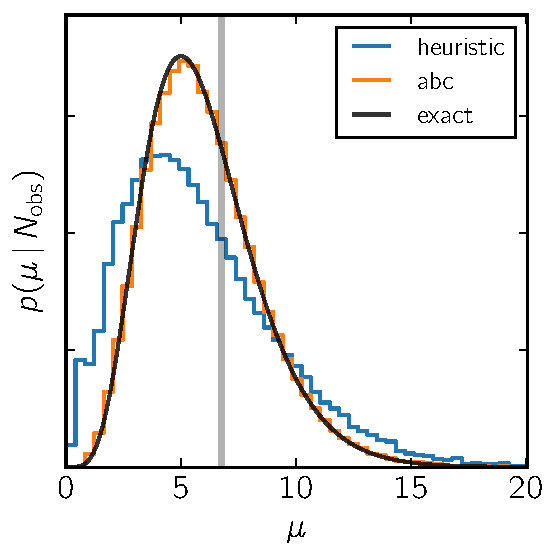
\includegraphics{figures/abctoy.pdf}
\end{center}
\caption{%
A comparison between a commonly used heuristic method for doing inference with
stochastic models and \abc.
The blue histogram shows the posterior inference for the rate parameter $\mu$
using the heuristic likelihood function from \eq{heuristic-likelihood}, the
orange histogram shows the \abc\ inference using the pseudo-likelihood from
\eq{pseudo-likelihood}, and the black curve shows the exact posterior from
\eq{exact-posterior}.
The vertical gray line shows the true value of $\mu$ that was used to generate
the data.
\dfmfiglabel{abctoy}}
\end{figure*}


\section{A short introduction to Approximate Bayesian Computation}

The problem statement for \abc\ is that you have a method of (stochastically)
simulating representative data from the model given a set of parameters but it
is computationally intractable to compute the likelihood of a given data set
conditioned on these same parameters.
In other words, you can sample $D_\simu \sim p(D_\simu\mid\theta)$ but you
can't directly evaluate $p(D_\obs\mid\theta)$ for any values $D_\obs$ and
$\theta$.
This means that you can't use standard \mcmc\ methods to draw samples from the
posterior probability $p(\theta\mid D_\obs) \propto
p(D_\obs\mid\theta)\,p(\theta)$.

To motivate \abc, let's start with an extreme method.
Let's say that sample a set of parameters $\theta \sim p(\theta)$ from your
prior and then simulate some data $D_\simu$ that just happens to
\emph{exactly} match the observed data $D_\obs$.
In this case, under your simulation model, this value of $\theta$ is a valid
sample from the posterior probability density $p(\theta\mid D_\obs)$ even
though you never evaluated the likelihood.
Now if you had an infinite amount of computing power and could draw a huge
number of samples following this procedure and rejecting all samples that
don't result in an exact match for your data then you could produce a
posterior sampling for $p(\theta\mid D_\obs)$ without ever evaluating the
likelihood.
Of course this method is absurd and intractable so \abc\ builds on this using
two observations
\begin{enumerate}
\item This method will still be correct if sufficient statistics of the
simulated data match the same sufficient statistics on the observed data.
\item The comparison between the simulation and the observation can be
``softened'' without significant loss of information.
\end{enumerate}
The first point is correct by definition but we will return to the relevant
subtleties below.
The second point is less obvious.

\begin{itemize}
\item Qualitative justification.
\item Theoretical basis.
\item Methodological questions: (a) sufficient statistics, (b) distance
function, (c) inference algorithm.
\end{itemize}


\section{The occurrence rate of small and cool exoplanets}

\begin{itemize}
\item Sample selection \citep{Burke:2015}.
\item Generative model: power laws, discussion of Poisson process.
\item Observation model: \citep{Christiansen:2013,Christiansen:2015,Burke:2015}
\item Statistics, distance metric
\item Inference method: PMC, MCMC, etc.
\item Results: compare to \citet{Burke:2015}
\end{itemize}

\section{The multiplicity \& mutual inclination of exoplanetary systems}

\begin{itemize}
\item Sample selection: looks as a function of stellar type.
\item Generative model: more flexible than power laws.
\item Observation model: calibrating the completeness and caveats: CITE
Christiansen note
\item Inference method: PMC, MCMC, etc.
\item Results
\end{itemize}

\section{The potential impact of Approximate Bayesian Computation}

\begin{itemize}
\item More general generative models means fewer and weaker assumptions.
\item False positives.
\item Physical models.
\end{itemize}


\vspace{1.5em}
All of the code used in this project is available from
\url{https://github.com/dfm/exoabc} under the MIT open-source software
license.
This code (plus some dependencies) can be run to re-generate all of the
figures and results in this \paper; this version of the paper was generated
with git commit \texttt{\githash} (\gitdate).

% \acknowledgments
\vspace{1.5em}
DFM would like to thank Jessi Cisewski for introducing him and the SAMSI
exoplanet populations working group to the method of \abc.
It is a pleasure to also thank
Eric Agol,
Eric Ford,
David Hogg,
and
Richard Wilkinson,
for helpful discussions and contributions.

\dfmtodo{Thank SAMSI.}

This research made use of the NASA \project{Astrophysics Data System} and the
NASA Exoplanet Archive.
The Exoplanet Archive is operated by the California Institute of Technology,
under contract with NASA under the Exoplanet Exploration Program.

This \paper\ includes data collected by the \kepler\ mission. Funding for the
\kepler\ mission is provided by the NASA Science Mission directorate.
We are grateful to the entire \kepler\ team, past and present.
Their tireless efforts were all essential to the tremendous success of the
mission and the successes of \ktwo, present and future.

These data were obtained from the Mikulski Archive for Space Telescopes
(MAST).
STScI is operated by the Association of Universities for Research in
Astronomy, Inc., under NASA contract NAS5-26555.
Support for MAST is provided by the NASA Office of Space Science via grant
NNX13AC07G and by other grants and contracts.

Computing resources were provided by High Performance Computing at New York
University.

\facility{Kepler}
\software{%
    \project{corner.py} \citep{Foreman-Mackey:2016},
	\project{matplotlib} \citep{Hunter:2007},
	\project{numpy} \citep{Van-Der-Walt:2011},
	\project{scipy} \citep{Jones:2001}
}

% \newpage
% \appendix
% \section{Appendix}


\bibliography{exoabc}

\end{document}
